%
\documentclass[10pt,a4paper]{article}


\usepackage{array}
\usepackage{subfigure}
\usepackage{graphicx}
\usepackage{amssymb}
\usepackage{amsmath}
\usepackage{cite}
\usepackage{color}
\usepackage{url}
\usepackage[lined,linesnumbered,ruled,norelsize]{algorithm2e}
\usepackage{listings}
\lstset{
  language=Octave, 
  basicstyle=\footnotesize, 
  frame=single, 
  showspaces=false, 
  showstringspaces=false}
\date{}




\begin{document}

\title{Technical Report 2: Multivariate Linear Regression}

\maketitle

\section{Selecting Learning Rate}
%
  We try six learning rates in our experiments, and the results are demonstrated in Fig.~\ref{fig:con}. It is shown that, if we take a very small learning rate (e.g., 0.01), the cost function is decreased very slowly, which means slow convergence during the gradient descent. Mover, when the learning rate is increased (e.g., from 0.01 to 1), the algorithm is of faster convergence. But, if a excessively large learning rate is adopted (e.g., 1.3), the convergence speed is no longer increased. In summary, we have to carefully tune the learning rate in our algorithm.
  %
  \begin{figure}[htb!]
  \centering
    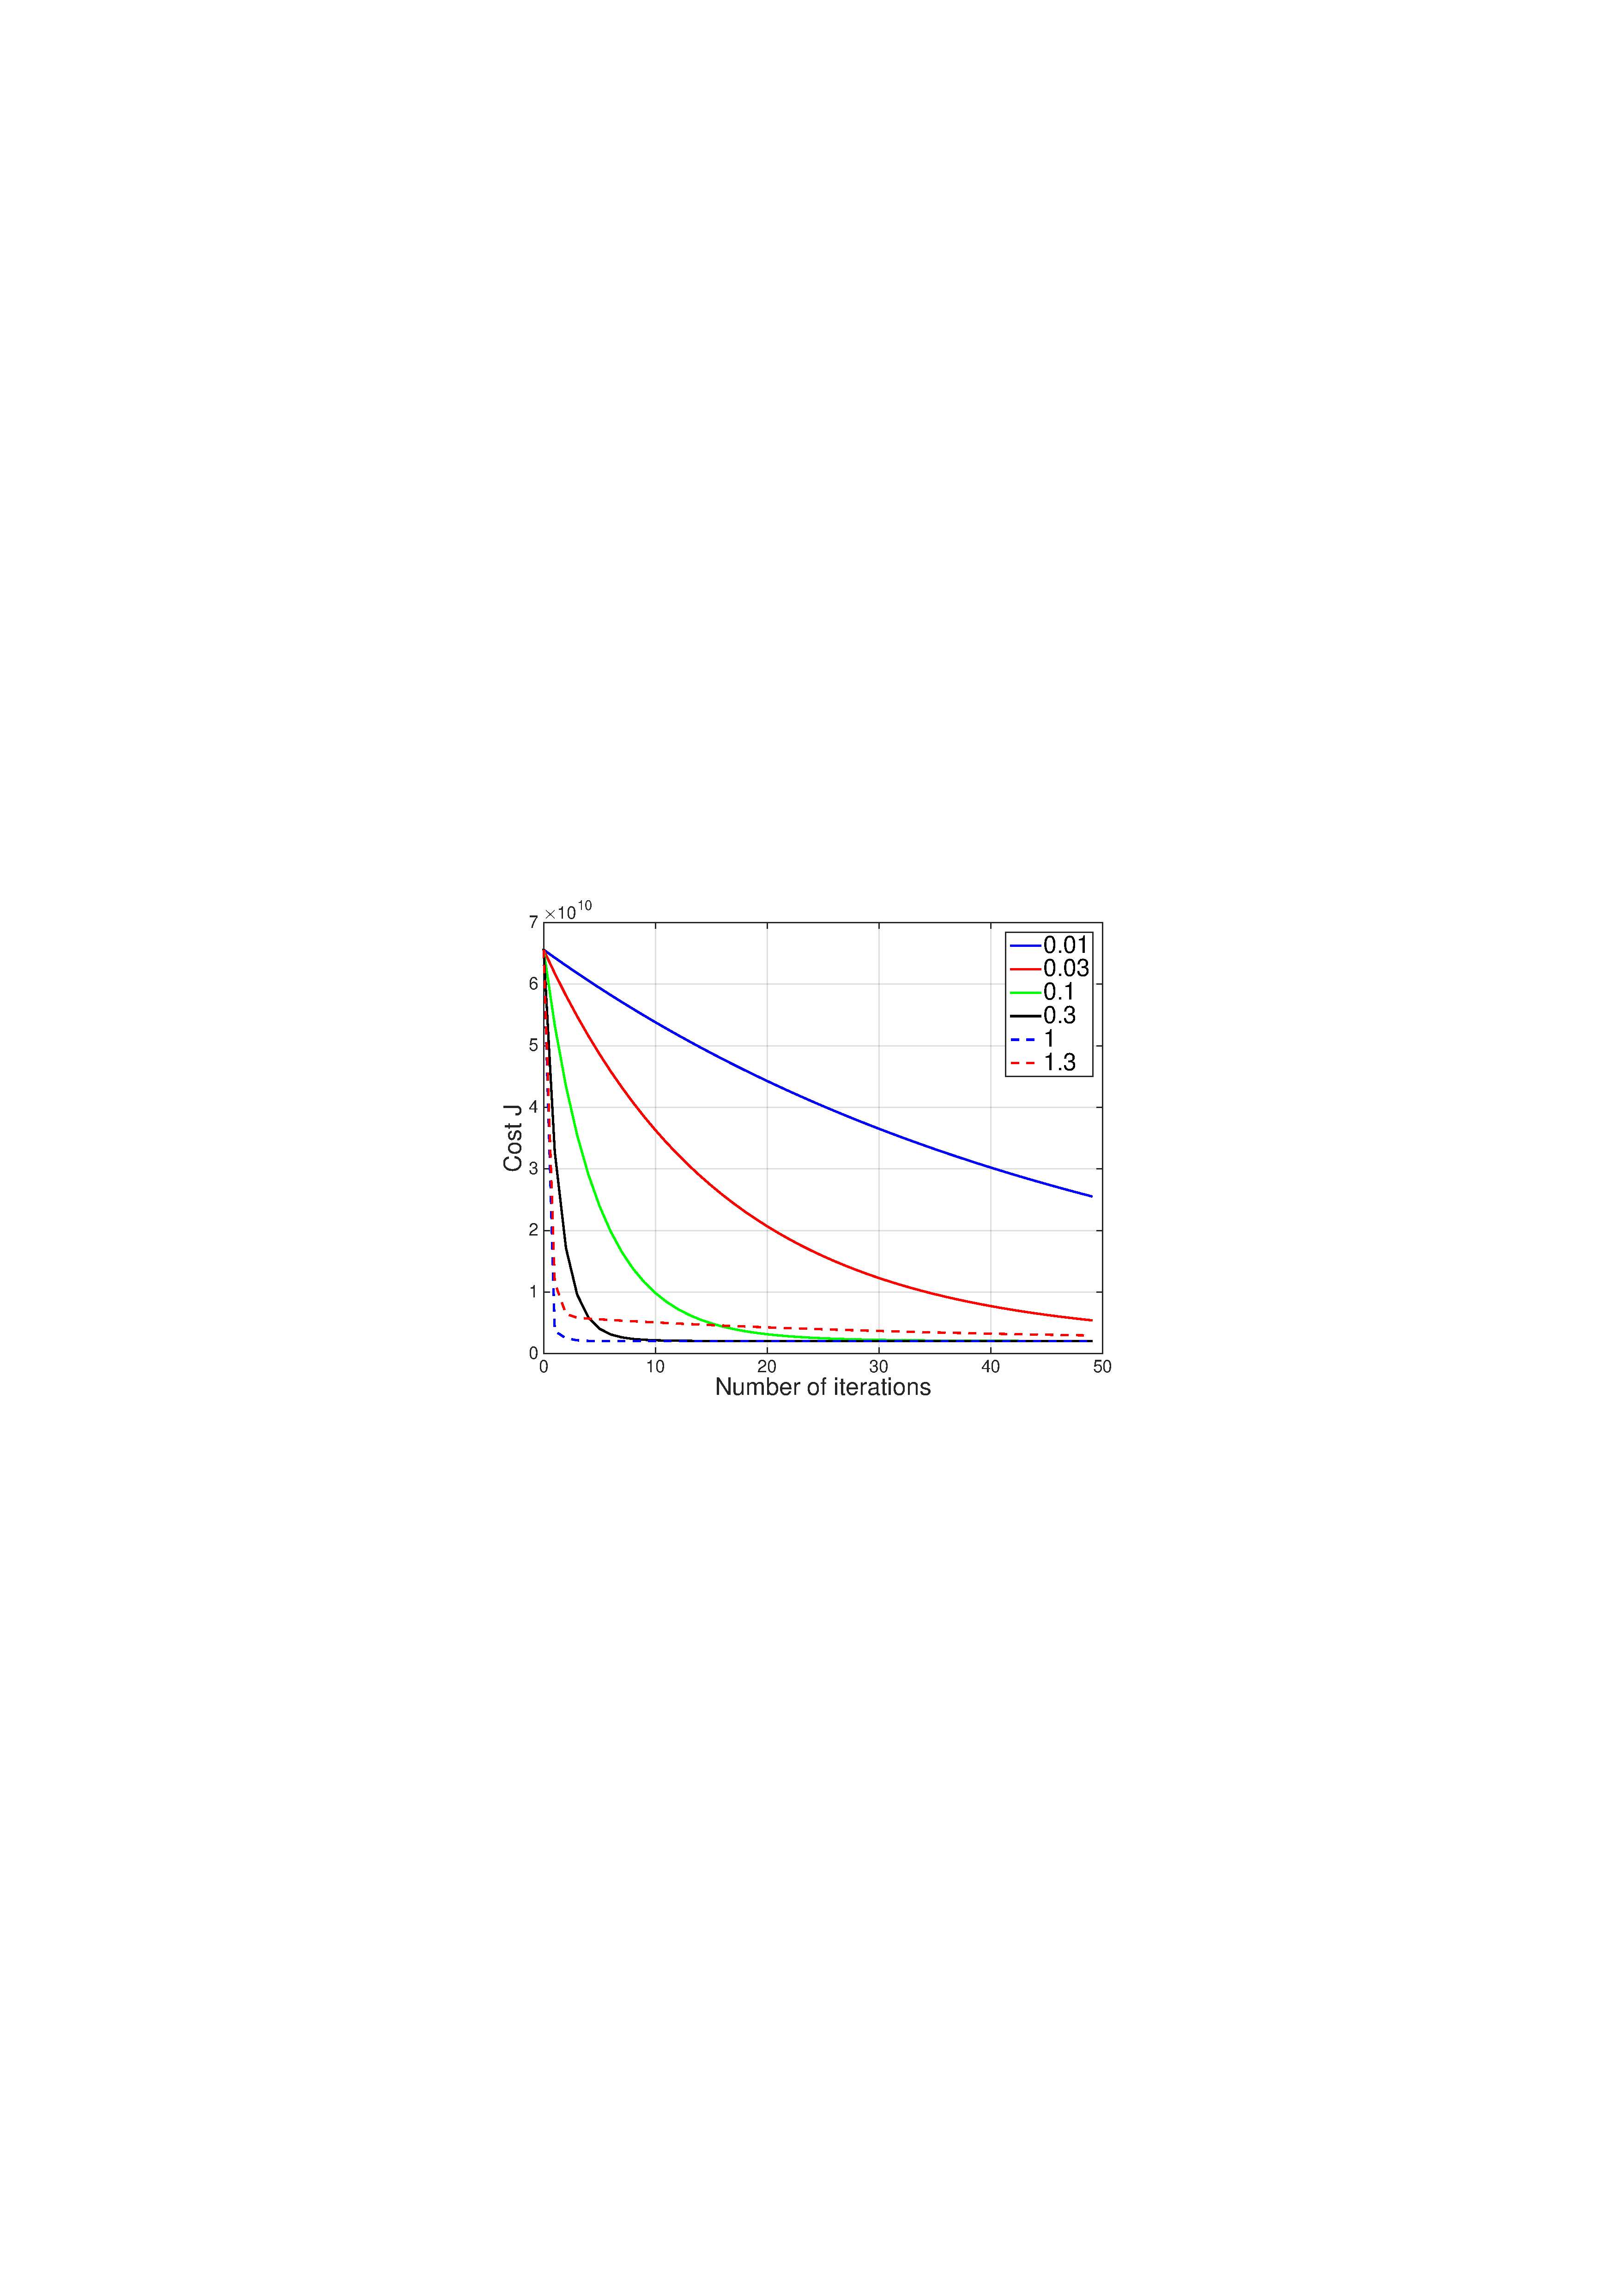
\includegraphics[width=.6\columnwidth]{convergence} \\ %\vspace{1ex}
  \caption{Convergences under different learning rates.}
  \label{fig:con}
  \end{figure}

  Apparently, $\alpha=1$ is the best choice, and we have $\theta_0=340413$, $\theta_1=110631$, $\theta_2=-6649$. Withe the above setting of $\theta$, we can predict the price of the given house which is 1650 square feet and 3 bedrooms. According to our calculation, the predicted price of the house should be \$293,081.

\section{Normal Equations}
%
  For the normal equations, the values of $\theta$ should be $\theta_0 = 89598$, $\theta_1=139.21$, and $\theta_2=-8738.0$. Notice that these values are different from the ones you got from gradient descent. This is because features don't need to be scaled when using the normal equations solution. The predicted price of the house should be \$293,081, as before.
  

\end{document}








  \end{lstlisting}
  %


